\documentclass{article} % Класс печатного документа

\usepackage{svg} % Вставка svg картинок (используется incscape)
\usepackage[utf8]{inputenc} % Кодировка исходного текста - utf8
\usepackage[english,russian]{babel} % Поддержка языка - русского с английским
\usepackage{tabularx} % Для создания таблицы во всю ширину текста
\usepackage{xcolor,colortbl} % Для определения цвета

\setsvg{svgpath = tree/}

% Отключение отступа перед новым параграфом
\setlength\parindent{0pt}

% Определение серого цвета для колонки
\definecolor{Gray}{gray}{0.85}

% Переопределение X типа колонки, чтобы был выровнен по вертикали по центру
\renewcommand{\tabularxcolumn}[1]{>{\small}m{#1}}
% Определение колонки выровненной по центру на оставшееся место по ширине
\newcolumntype{Y}{>{\centering\arraybackslash}X}
% Определение серой колонки
\newcolumntype{g}{>{\columncolor{Gray}}c}

\begin{document} % Конец преамбулы, начало текста
\textbf{Студент:} Свичкарев Анатолий Владленович

\textbf{Ген:}
\begin{center}
	\begin{tabularx}{\textwidth}{|g|Y|} \hline
		Названиe & \textbf{P53} (Также известен как: CG10873; CG31325;
			   CG33336; D-p53; Dm-P53; Dmel\textbackslash CG33336;
			   dmp53; Dmp53; DmP53; DMP53; dp53; Dp53; prac) \\ \hline
		Расположение на хромосоме & Chr: 3R, 23049657..23054082,
			   		    комплементарная цепь (Релиз 6.01)\\ \hline
		Функция & белок кодирующая (контроль апоптоза,
			  деление клетки и пролиферация)\\ \hline
	\end{tabularx}
\end{center}

\textbf{Организмы:} 
\begin{center}
\begin{tabularx}{\textwidth}{|g|Y|Y|Y|Y|Y|} \hline
	\rowcolor{Gray}
	\# & Названиe (лат) & Названиe (рус) & Длина транскрибируемой области & Длина белка & Позиции экзонов \\ \hline
	1 & Drosophila melanogaster & Плодовая мушка & 1577 & 1551 & 689..726, 884..964, 1035..1071, 1135..1161, 2959..3268, 3333..3579, 3642..4036, 4096..4118 \\ \hline
	2 & Drosophila simulans & Плодовая мушка & 1215 & 1215 & 1..1215 \\ \hline
	3 & Drosophila sechellia & Плодовая мушка & 1215 & 1215 & 1..1215 \\ \hline
	4 & Drosophila erecta & Плодовая мушка & 1215 & 1215 & 1..1215 \\ \hline
	5 & Drosophila mauritiana & Плодовая мушка & 1215 & 1215 & 1..1215 \\ \hline
	6 & Drosophila yakuba & Плодовая мушка & 1215 & 1215 & 1..1215 \\ \hline
	7 & Drosophila pseudoobscura pseudoobscura & Плодовая мушка & 1215 & 1215 & 1..1215 \\ \hline
	8 & Drosophila persimilis & Плодовая мушка & 1215 & 1215 & 1..1215 \\ \hline
\end{tabularx}
\end{center}

\pagebreak
\textbf{Визуальные результаты поиска BLASTN:}

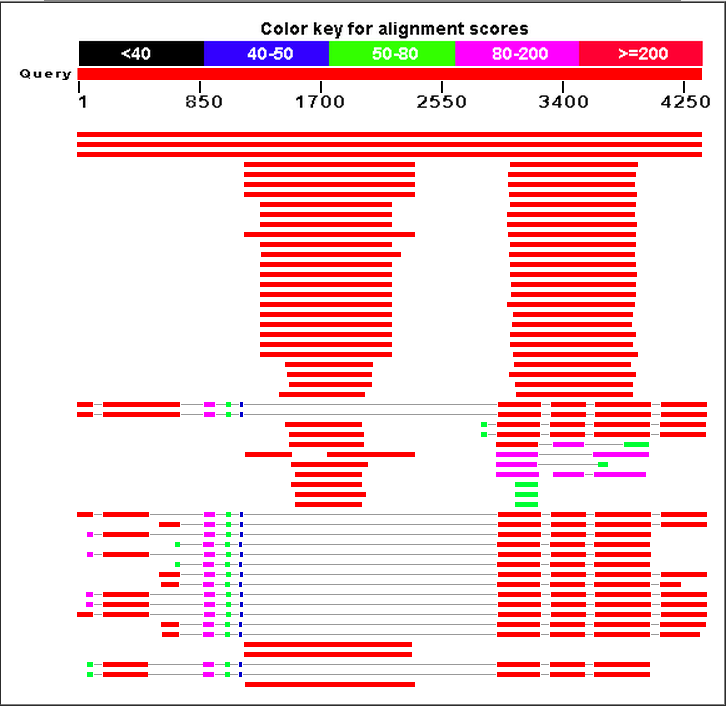
\includegraphics[width=\textwidth]{blastn_align}

\textbf{Артефакты выравнивания:}

файл с выравниваниями - alignment.fa

Блок 1 – можно поставить gap перед T в первой последовательности, тогда
выравнивание будет лучше.

Блок 2 – можно три C в первых последовательностях ближе к концу сместить
правее под нижние C.

Блок 3 – можно две первых A в последних последовательностях сместить влево
с gap, чтобы выровнять с A из первой последовательности.

\textbf{Выбор блоков:}

\begin{center}
\begin{tabularx}{\textwidth}{|g|Y|Y|} \hline
	\rowcolor{Gray}
	\# & Позиции во множественном выравнивании & Длина \\ \hline
	1 & [518..527] & 10 \\ \hline
	2 & [2082..2084] & 13 \\ \hline
	3 & [4217..4229] & 12 \\ \hline
\end{tabularx}
\end{center}

\pagebreak
\textbf{Филогенетические деревья для полного выравнивания:}

\textbf{Minimum-evolution:}

\textbf{Maximum likehood:}

\textbf{Neighbor-Joining:}

\begin{figure}[h]
	\includesvg[width=\textwidth]{image2}
\end{figure}

\textbf{Филогенетические деревья для каждого фрагмента \mbox{выравнивания}:}

\textbf{Фрагмент 1:}

\textbf{Minimum-evolution:}

\textbf{Maximum likehood:}

\textbf{Neighbor-Joining:}


\textbf{Фрагмент 2:}

\textbf{Minimum-evolution:}

\textbf{Maximum likehood:}

\textbf{Neighbor-Joining:}


\textbf{Фрагмент 3:}

\textbf{Minimum-evolution:}

\textbf{Maximum likehood:}

\textbf{Neighbor-Joining:}

\end{document} % Конец документа
